%\usepackage[utf8]{inputenc}
\usepackage[T1]{fontenc}
\usepackage[brazil]{babel}
\usepackage{csquotes}
\usepackage{microtype}
\usepackage{lmodern}
\usepackage{indentfirst}
%\usepackage{parskip} % sem indentações
\usepackage[onehalfspacing]{setspace}
\usepackage[lmargin=3cm,tmargin=3cm,rmargin=2cm,bmargin=2cm,headheight=28pt]{geometry} % [showframe]
\usepackage[output-decimal-marker={,},per-mode=symbol]{siunitx}

\usepackage{lipsum}
\setlipsumdefault{1}

\usepackage{graphicx}
\usepackage{multicol,multirow}
\usepackage{booktabs}
\usepackage{titlesec}
\usepackage{caption}
\usepackage{subcaption}
\usepackage{hyperref}
\usepackage{tocloft}
\usepackage{enumitem}
\usepackage{adjustbox}
\usepackage{float}
\floatstyle{plaintop}
\restylefloat{table}

%%%%%%%%%%%%%%%%%%%%%%%%%%%%%%%%%%%%%%%%%%%%%%%%%%%%%%%%%%%%
%  Adiciona pontos nas seções no sumário (classe article)  %
%%%%%%%%%%%%%%%%%%%%%%%%%%%%%%%%%%%%%%%%%%%%%%%%%%%%%%%%%%%%

\renewcommand\cftsecfont{\normalfont}
\renewcommand\cftsecpagefont{\normalfont}
\renewcommand{\cftsecleader}{\cftdotfill{\cftdotsep}}

%%%%%%%%%%%%%%%%%%%%%%%%%%%%%%%%
%  referencias bibliográficas  %
%%%%%%%%%%%%%%%%%%%%%%%%%%%%%%%%
\usepackage[backend=biber,style=abnt,giveninits]{biblatex} %

\usepackage{fancyhdr}
\fancyhf{}
\pagestyle{fancy}
\lhead{
\includegraphics[height=0.8\headheight]{C:/users/victo/OneDrive/GitHub/latex/figuras/ucam-header.png}}
\fancyhead[RO]{\thepage}
\renewcommand{\headrulewidth}{0.8pt}

\newlist{enumalpha}{enumerate}{1}   % Cria um novo ambiente enumerate com letras
\setlist[enumalpha]{label=\alph*)}  % pode-se criar vários sem alterar o original

\usepackage{color}   %May be necessary if you want to color links

\hypersetup{
    colorlinks=true, %set true if you want colored links
    linktoc=all,     %set to all if you want both sections and subsections linked
    linkcolor=blue,  %choose some color if you want links to stand out
    citecolor=black,
    urlcolor=blue
}


\documentclass[a4paper,12pt]{article}
\usepackage[utf8]{inputenc}
\usepackage[T1]{fontenc}
\usepackage[brazil]{babel}
\usepackage[tmargin=2cm,lmargin=3cm,rmargin=2cm,bmargin=2cm]{geometry}
\usepackage{amsmath, amssymb, mathtools}
\usepackage[output-decimal-marker={,},per-mode=symbol]{siunitx}
\usepackage{enumitem}
\usepackage{microtype}

\usepackage{todonotes}
\reversemarginpar
\setlength{\marginparwidth}{2cm}
\author{Victor Locatelli}
\title{}
\date{}

\begin{document}

%%! TEX root = ../listas_completas.tex

%%%%%%%%%%%%%%
%  EQUAÇÕES  %
%%%%%%%%%%%%%%

\section{Equações:}% \label{sec:equacoes_}
\begin{equation}\label{eq:zeta}
\zeta=\frac{c}{c_{c}}
\end{equation}
\begin{equation}\label{eq:Cc}
c_{c}=2 m \sqrt{\frac{k}{m}}=2 \sqrt{k m}=2 m \omega_{n}
\end{equation}
\begin{equation}\label{eq:xt}
    x_{t}=A_{1} e^{\lambda_{1} t}+A_{2} e^{\lambda_{2} t}
\end{equation}
Em que $\lambda_1$ e $\lambda_2$ são calculados com a equação~\ref{eq:lambda}
abaixo:
\begin{equation}\label{eq:lambda}
\lambda_{1,2}=\omega_{n}\left(-\zeta\pm \sqrt{\zeta^{2}-1}\right)
\end{equation}
Ou ainda da forma expandida:
\begin{equation}\label{eq:xt_expandida}
x_{t}=A_{1} e^{\left[\omega_{n}(-\zeta+\sqrt{\zeta^{2}-1})\right] t}+A_{2} e^{\left[\omega_{n}(-\zeta-\sqrt{\zeta^{2}-1})\right] t}
\end{equation}

\begin{itemize}
    \item Sistema Superamortecido: $\zeta > 1$
    \item Sistema criticamente amortecido: $\zeta = 1$
    \item Sistema sub-amortecido: $\zeta < 1$
\end{itemize}



\begin{figure}[ht]
    \centering
    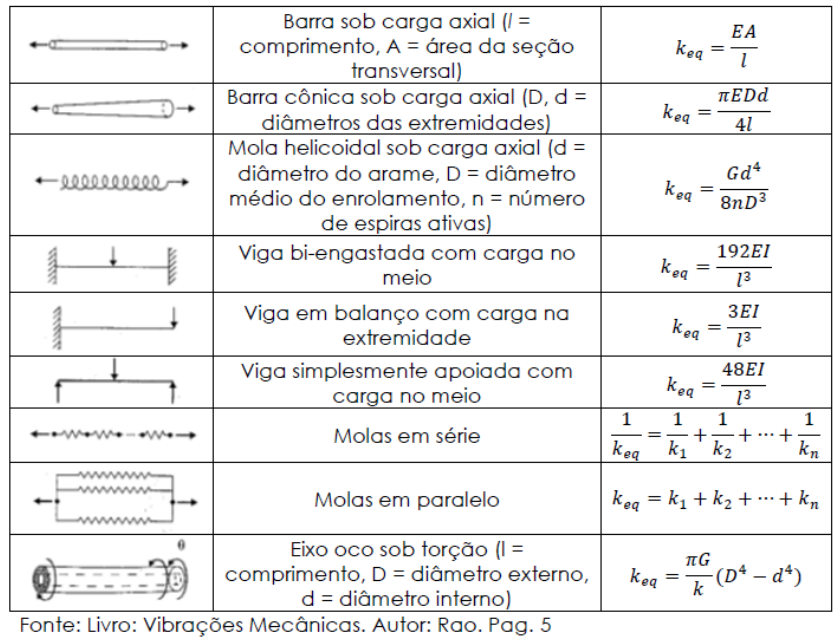
\includegraphics[width=0.8\textwidth]{imagens/rigidez_equivalente.png}
    \caption{Rigidez equivalente}
    \label{fig:rigidez_equivalente}
\end{figure}
\begin{figure}[ht]
    \centering
    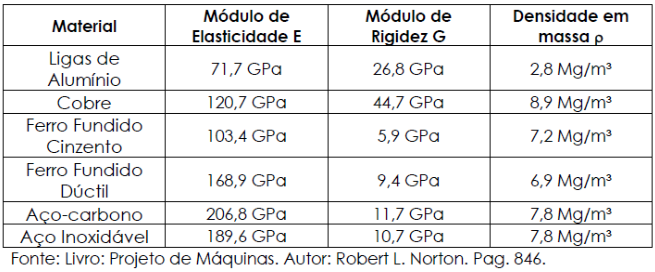
\includegraphics[width=0.8\textwidth]{imagens/propriedades_materiais.png}
    \caption{Propriedades de alguns materiais}
    \label{fig:propriedades_materiais}
\end{figure}

\begin{figure}[ht]
    \centering
    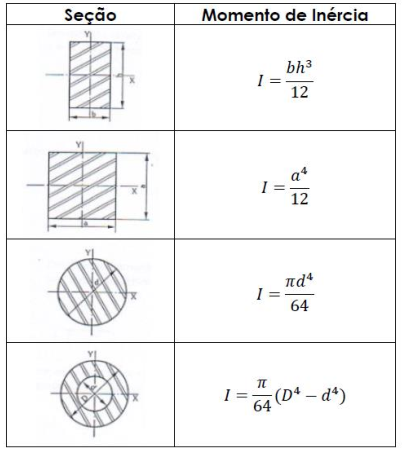
\includegraphics[width=0.5\textwidth]{imagens/momento_de_inercia.png}
    \caption{Momento de inércia}
    \label{fig:imagens-momento_de_inercia-png}
\end{figure}

\section{Equações:}% \label{sec:equacoes_}

\subsection{Associação de molas em paralelo}

\begin{equation}k_{e q}=\sum_{i=1}^{n} k_{i}\end{equation}

\subsection{Associação de molas em série}
\begin{equation}\frac{1}{k_{e q}}=\frac{1}{k_{1}}+\frac{1}{k_{2}}+\cdots+\frac{1}{k_{n}}\end{equation}

\section{Vibração livre com amortecimento viscoso}%
\label{sec:vibracao_livre_com_amortecimento_viscoso}

\subsection{Frequência natural}
\begin{equation}
    \omega_n = \sqrt{\frac{k}{m}} = \si{\radian\per\second}
\end{equation}

\subsection{Fator de amortecimento}%
\label{sub:fator_de_amortecimento}

\begin{equation}\label{eq:zeta}
\zeta=\frac{c}{c_{c}}
\end{equation}

\begin{equation}\label{eq:Cc}
c_{c}=2 m \sqrt{\frac{k}{m}}=2 \sqrt{k m}=2 m \omega_{n}
\end{equation}

\subsection{Solução Geral}%
\label{sub:solucao_geral}

\begin{equation}\label{eq:xt}
    x_{t}=A_{1} e^{\lambda_{1} t}+A_{2} e^{\lambda_{2} t}
\end{equation}
Em que $\lambda_1$ e $\lambda_2$ são calculados com a equação~\ref{eq:lambda}
abaixo:

\begin{equation}\label{eq:lambda}
\lambda_{1,2}=\omega_{n}\left(-\zeta\pm \sqrt{\zeta^{2}-1}\right)
\end{equation}

Ou ainda da forma expandida:

\begin{equation}\label{eq:xt_expandida}
x_{t}=A_{1} e^{\left[\omega_{n}(-\zeta+\sqrt{\zeta^{2}-1})\right] t}+A_{2} e^{\left[\omega_{n}(-\zeta-\sqrt{\zeta^{2}-1})\right] t}
\end{equation}

\begin{itemize}
    \item Sistema Superamortecido: $\zeta > 1$
    \item Sistema criticamente amortecido: $\zeta = 1$
    \item Sistema sub-amortecido: $\zeta < 1$
\end{itemize}

\end{document}
